\selectlanguage{english}
\chapter{Squirrel: Architecture Driven Resource Management}
\label{chp:squirrel}
\markboth{Squirrel: Architecture Driven Resource Management}{Chapter5}

%\coolphrase {
%	I still don't know
%}{Some name here}


%Resource management is critical to guarantee Quality of Service when various stakeholders share the execution environment, such as cloud or mobile environments.
%In this context, providing management techniques compatible with standard practices, such as component models, is essential.
%Resource management is often realized through monitoring techniques, while resource isolation uses virtual machines or containers (e.g., docker).
%These techniques (i) impose varying levels of overhead depending on the managed resource, and (ii) are applied at different abstraction levels, such as processes, threads or objects.
%Thus, mapping components to system-level abstractions in the presence of resource management requirements can lead to sub-optimal systems.
%
%We propose Squirrel, an approach to tune component deployment and resource management in order to reduce management overhead.
%At runtime, Squirrel uses an architectural model annotated with resource requirements to guide the mapping of components to system abstractions, providing different resource management capabilities and overhead.
%We present an implementation of Squirrel, using a Java component framework,
%and a set of experiments to validate its feasibility and overhead.
%We show that choosing the right \textit{component-to-system} mappings at deployment-time reduces performance overhead and/or memory use.

\section{Introduction}

Resource management is critical for domains where software components share an execution environment but belong to different stakeholders.
For instance, in multi-tenant systems resource management is used to guarantee safety, reliability and per-stakeholder Quality of Service (QoS).
These applications essentially require the isolation of tenants in terms of resource consumption~\cite{KrWeKo2013-icwe-MTBenchmark}.
This enables, for example, \textit{Software-as-a-Service} layers for cloud systems, allowing innovative pricing policies based on user requirements. %(e.g. user A has a \textit{premium} contract that guarantees a response time inferior to 500 ms for each request, while user B has a \textit{standard} contract that does not guarantee any response time).
Since these services are often implemented on paradigms such as component models,
the design of resource management techniques dedicated to component models is an important issue.

Component model implementations represent high level concepts, such as component instances, by means of mapping them to system-level abstractions like objects, threads, processes or virtual machines.
Each mapping has unique features in terms of performance, memory footprint, etc.
However, these mappings are often done in a once-size-fits-all manner, allowing some choices to optimize for memory use while others might, for example, improve inter-component communication.
%\hl{The mapping of components to system abstractions, which has the goal of improving some parameters of the runtime, has often been made in a homogeneous way for all components.[I DON'T UNDERSTAND?, Quiero decir que todos los componentes usan el mismo mapping, todos son representados como hilos, o todos como procesos. La parte de ``som parameters'' significa que cuanod se toma esa decision durante la implementacion del framework se hace con un objetivo como reducir el uso de memoria o facilitar la comunicacion entre componentes o garantizar un ``sandbox'' para los componentes]}
Interestingly, system abstractions offer varying resource management capabilities that differ in how they impact the application.
Although we can hard-code the resource management concern during the design of the component model, we argue that this leads to sub-optimal systems with high  overhead~\cite{binder_portable_2006,czajkowski_jres:_1998,Maurel:2012:AME:2304736.2304763} because components have different resource requirements.

% without taking into account resource management concerns, and (ii) .

To address this issue, we propose Squirrel, an approach to resource management for component models that aims at reducing overhead.
In Squirrel, the application is deployed with a model containing resource usage contracts for each component and a detailed view of the system.
These metadata are used to choose at deployment-time the best way of representing each component in terms of system abstractions.
This contrasts with the \textit{traditional} approach of binding the representation during the design of the component model and results in the final runtime representation of the system only being known after deployment.
%uses meta-data regarding the application's structure and its requirements to deploy components on system-level abstractions.



%During deployment, the information is used to automatically create a new deployment model where components are automatically mapped into abstractions that we call \textit{containers}.
%Each \textit{container} is then configured based on the components' resource contracts, ensuring resource consumption while minimizing the overhead.

In this paper we discuss an approach to resource management applicable to any component model. To validate the feasibility of our proposal, we present a reference implementation for a Java-based component model.
A set of experiments validate its feasibility and show various aspects of its overhead.
The results demonstrate that choosing the right \textit{component-to-system} mappings at deployment-time can reduce performance overhead and/or memory footprint.
%\hl{INTI: Se que esta oracion es muy general, el problema es que no estoy seguro de si poner los numeros es lo correcto pues los ejemplos son tan solo para mostrar con un caso de uso los potenciales beneficios de postergar la decision acerca de como hacer el manejo de recursos.}
The contributions of this paper are as follow:
\begin{itemize}
\item An approach for architecture driven resource management that leverages structural information to guide the mapping of component model concepts onto system-level abstractions.
\item A reference implementation of the Squirrel framework for a Java-Based component platform.
\item A performance comparison showing how different mappings can impact the overhead of the system and how the approach behaves in comparison to state-of-practice approaches for resource management.
\end{itemize}

The remainder of this paper is organized as follows.
The next section presents some foundational work we use along this paper.
Section \ref{sec:apprach} describes the Squirrel approach and presents how we leverage metadata to drive resource management.
In section~\ref{sec:kevoree} we propose a reference implementation of Squirrel for a Java-based component platform.
A validation of the implementation through a set of experiments is presented in section~\ref{sec:evaluation}.
Finally, section \ref{sec:related-works} discusses related work and section \ref{sec:conclusions} presents our conclusions and future work.


%\section{Background on resource management }

%\textbf{Synthesis.}
%Providing resource management features at the application level is possible, but it introduces high overhead in the application \cite{gonzalezherrera:hal-00983045}, thus greatly limiting its interest.
Current middleware either provide limited resource-awareness or totally hide resource concerns from the application.  Following the same ideas as in \cite{guerraoui1999oo} where authors explain that the distribution concern should not be hidden from developers in object-oriented distributed programming, we believe that the resource management concern should not be hidden from application developers. We envision combining monitoring techniques and system-layer resource management techniques to achieve this goal. 
This section presents a summary of two underlying techniques used to monitor and reserve resources. 



%These approaches are used in section~\ref{sec:kevoree}.

%Providing adequate support for pervasive applications is a challenge because their resource requirements vary (e.g., processors, memory bandwidth, I/O).
%For critical applications, such as surveillance systems, a known bounded amount of resources must be guaranteed for the application to run properly. For multimedia applications, the amount of required resources may change over time and dynamic adaptations and redeployment can be required. 

%Lots of modern middleware are typically implemented using Java (for example with OSGi) because of its safety, flexibility, and mature development environment.
%However, the Java virtual machine was designed to execute a single application at a time and does not provide \textit{per-component} resource reservation.
%Current Java-based middleware are thus unable to reserve resources for critical applications, which may cause these applications to crash or hang when insufficient resources are available.

%As an example, we can consider a smart home system that simultaneously provides services that are critical for user safety, and services that increase user comfort. 
%For example, a smart home system can provide a health monitoring service for elderly people allowing them to stay at home while regularly reporting on their health and quickly raising alarms in case of emergency. 
%The same system can simultaneously provide services for closing all shutters at night or to access multimedia content.
%All these services constantly evolve after their initial deployment and thus their behavior and requirements regarding resource consumption may change accordingly.
%For these environments, where services featuring various degrees of criticality share the same execution environments and thus the same resources, a mechanism to guarantee resource access and priority is required.

\textbf{Cgroups} (control groups) is a Linux kernel feature to limit, account, and isolate the resource usage of processes. 
It provides a low-level API to access properties on resource usage that allow to i) limit memory consumption per task, 
ii) assign a minimum percentage of CPU time to the task,
iii) establish a minimum and maximum throughput for I/O block devices and network throughput per task, and
iv) measure the resources a task uses.
Cgroups are used in particular in the context of lightweight process virtualization (e.g., OpenVZ, LXC).


\textbf{Scapegoat} provides an application-level adaptive resource monitoring framework~\cite{gonzalezherrera:hal-00983045}.
Each component is augmented with a contract that specifies its resource usage, such as peak CPU and memory consumption.
The framework adjusts the monitoring level to minimize overhead while still allowing precise accounting when needed.
The adjustment is done by selecting, through a heuristic, components that should be deeply monitored using intrusive instrumentation to check their contracts, while using a lightweight monitoring mode the rest of the time.
%Furthermore, Scapegoat proposed a heuristic that leverages information produced by the Models@runtime approach to quickly predict the faulty components.


%They are considered one of the building blocks to support Linux containers.



\section{Approach} \label{sec:apprach}

The main concept in Squirrel is the \textit{resource-aware container}.
Such containers are logical entities that take care of the resource management concern.
By logical we mean that it is not important, from a functional point of view, how a
container achieves resource management. 
Instead, a resource-aware container is an entity that \textit{wraps} a set of components and offers the following properties:
\begin{itemize}
\item \textbf{Resource consumption monitoring} refers to the ability to assess the 
quantity of resources used by a component.
\item \textbf{Resource reservation} is the capacity to ensure a given amount of
resources will be available whenever a component demands it.
\item \textbf{Resource isolation} guarantees that a component's behavior in terms
of resource usage does not interfere with the behavior of another component.
\end{itemize} 

%Even the idea of 
\textit{Wrapping} a set of components can be considered a soft definition because the \textit{membrane} of a resource-aware container limits the behavior
of the contained components only when it is relevant to the resource management concern.
For instance, components within different containers can still communicate directly
with each other through their interfaces without intervention of their containers as long as such communication does not affect the resource under management.  

In Squirrel we propose to automatically select, deploy and configure resource containers to manage resource usage.
The novelty is that we delay the selection of the container's implementation till deployment-time in order to have knowledge about the exact conditions of the system and thus minimize the overhead of the resource management system.
This idea is supported by the claim that components often require disjoint sets of resource types.
Our framework is composed of three essential elements: i) a mechanism to describe the management requirements of an application, ii) an admission control scheme in the middleware to handle the global view of resource availability, and iii) mechanisms to map component model concepts to system-level abstractions.
In the following subsections we describe our framework and its elements.

\subsection{Managing resources through architecture adaptations}
Modern application development models, such as component-based systems, promote the usage of Architecture Description Languages (ADL) or configuration models to check properties on the system's structure and to drive system deployment. 
In Squirrel, we propose to enhance this layer with metadata regarding resource reservation and to use these metadata to efficiently drive resource reservation offered at the system level.  
The idea is to follow a gray-box approach where we automatically adapt a component-based application by applying an architecture pattern to isolate a component within a resource-aware container.

\begin{figure}[htbp]
\centering
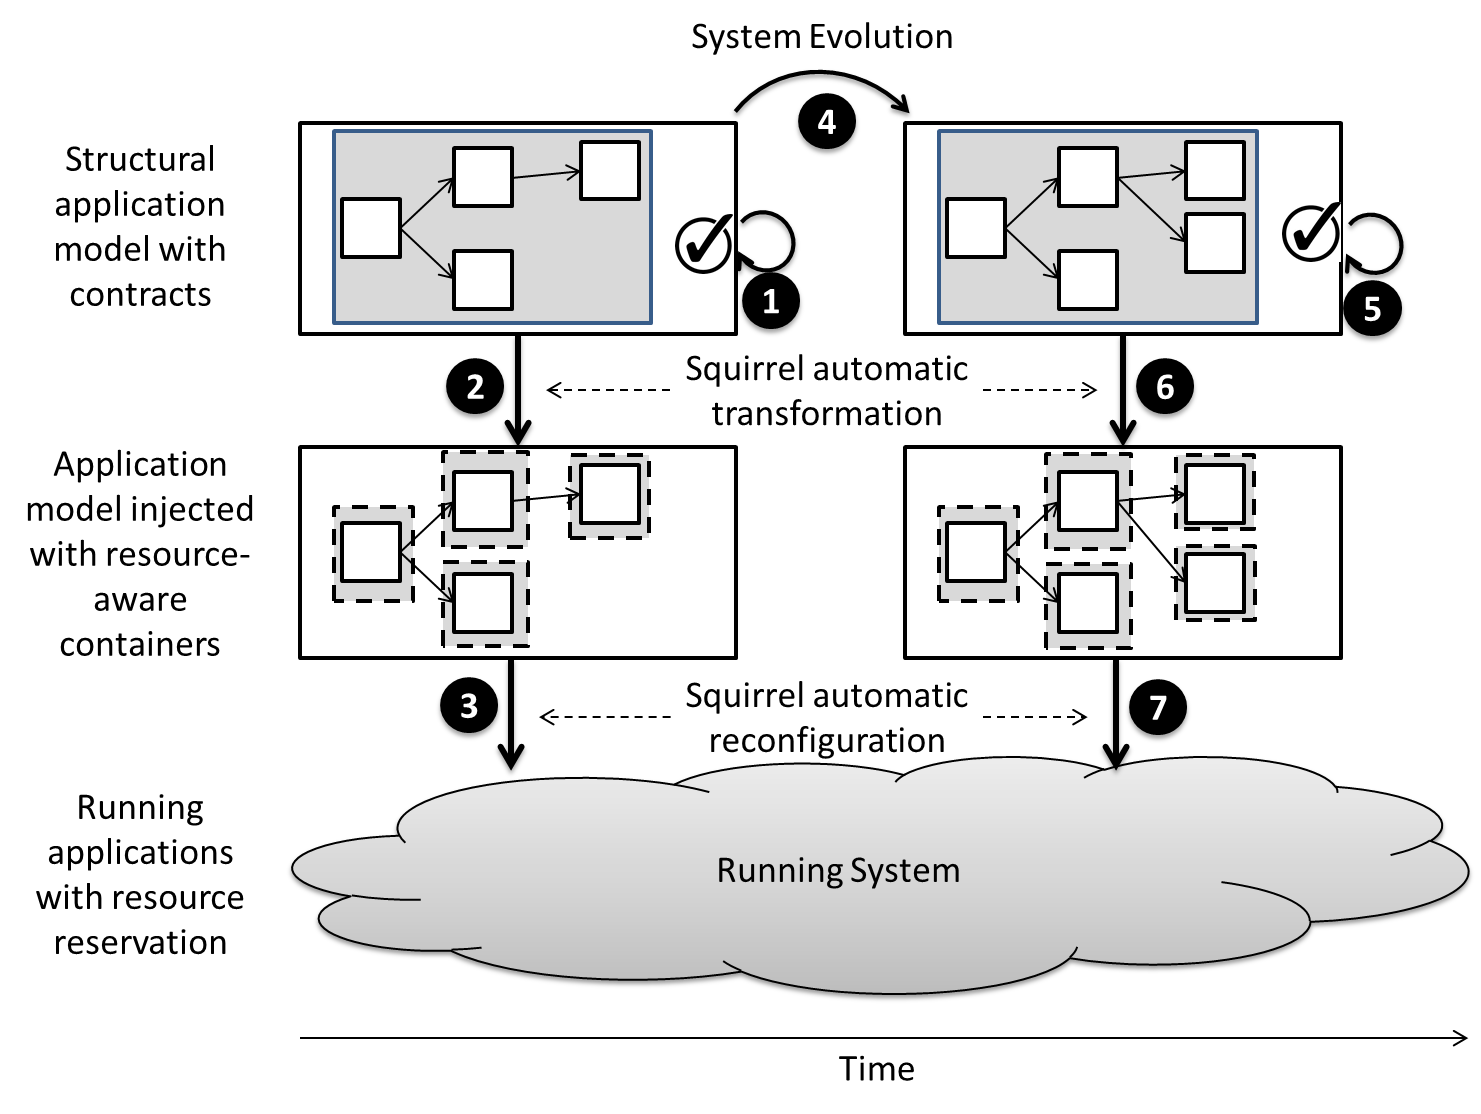
\includegraphics[width=0.7\textwidth]{chapter4/figures/globalOverview.png}
\caption{Squirrel approach for resources reservation} \label{fig:Overview}
\vspace{-0.5cm}
\end{figure}	

As illustrated in figure~\ref{fig:Overview}, Squirrel follows an automatic process to manage resources.
Squirrel receives an application's model, enhanced with contracts on resource reservation. 
Squirrel performs admission control to check the validity of the contracts on resource usage with respect to the available resources in the execution environment.
If the contracts are consistent with available resources, the process continues, if not, the application's model is refused.
Then, as depicted by arrow 2, Squirrel automatically transforms components or the configuration/architecture model by isolating components in resource-aware containers that can be finely configured to decrease the resource management overhead.
Finally, as depicted by arrow 3, Squirrel reconfigures the running system.
When the application evolves (arrow 4), 
%Squirrel automatically adapts the system while preserving resource reservation properties by applying the whole process on the new model (arrow 5, 6 and 7).
Squirrel attempts to preserve resource reservation properties while processing the new model (arrow 5, 6 and 7).


\subsection{Describing resource management requirements}
Beugnard et al. discuss the extending Meyer's \textit{Design-By-Contract} idea to software components~\cite{Beugnard774917}.
They classify component contracts into four categories: syntactic (level 1), semantic (level 2), synchronization (level 3), and Quality of Service (level 4).
%They explain that component contracts have to deal with concerns that they classified into 
%Fifteen years later, many component-based frameworks provide contracts that are used to: 
%i) Describe the component features with all required contracts.
%ii) Select from all contracts those that are useful in the context of component use, and configure them.
%iii) Evaluate contracts and react accordingly.
%iv) Decide when to stop evaluating contracts. 
There is no de-facto standard to describe component contracts, but many domain specific interface description languages contain such metadata.
This chapter assumes that components have contracts to deal with resource reservation (level 4).
A contract in Squirrel defines component resource requirements written in terms of resource types, quotas and expected component usage.
\begin{itemize}
\item{\textbf{Definition 1}} A resource type indicates any class of computational resource that is useful to a component.
Its consumption must be susceptible to monitoring and reservation.
In this paper, we consider CPU, Memory, Network Bandwidth and IO Throughput.

\item{\textbf{Definition 2}} Expected component usage describes the expected number of external invocations of each method of the component interface.
In short, let $C$ be a component instance, then $\forall{I \in C_{Interfaces}}, \forall{M \in I_{methods}} \\ {EU}_{IM}$ is the number of expected invocations of method $M$, per second.

\end{itemize}

A \textbf{contract in Squirrel} is a set of tuples with the form $\langle RT, N, MU \rangle$ where $RT$ is a resource type, N the maximum amount of resources to reserve, and $MU$ is the measuring unit used for this resource type.
Optionally, Squirrel supports the definition of a set of tuples with the form $\langle I, M, {EU}_{IM} \rangle$ where $I$ is a component interface, $M$ is a method of the interface, and ${EU}_{IM}$ the expected usage.
Implementations of the Squirrel approach must provide a way to define contracts with these concepts.
%In section~\ref{sec:kevoree} 
We use a domain-specific language to describe contracts.

\subsection{Admission control} \label{sect:admissionControl}

Providing resource reservation in a component based framework requires checking if components' resource-aware contracts are compatible with the resources available in the execution environment.
%The platform provides a fixed amount of resources that constitute the pool of resources used by components.
By checking the availability of resources, the platform controls component admissions.

%To support this dynamism while managing resources, 
To support resource management at runtime, Squirrel takes into account two events: i) component deployment, and ii) component removal.
%These are common operations on any middleware; hence adding a notification for these events is straightforward.
Whenever the application is modified, the system automatically recalculates the aggregated resources required by the application and compares it to the available resources in the execution environment.
If the available resources are greater than those required by the application, the reconfiguration is accepted, else, the application model is refused and the reconfigurations are discarded.

%\subsection{Defining multiple variants of execution model}
%\todo{I couldn't finish this, so I'm writing my ideas}
%To support our approach, a middleware needs to support multiple ways of mapping component instances into system/runtime abstractions.
%Somehow, it means that it needs an extension point to describe a factory for creating component instances.
%I can see two ways of doing so, either the writer of the middleware provides many versions of execution model or she provides a mechanism to extends the semantic of a component instance and of component containers (Node).
%In Kevoree we achieved this easily because it is naturally extensible, we can define new Node Types, New Channel Type, and we can compose them.
%Moreover, we use Models@Runtime to easily change between variant of mappings (e.g., we receive a model where each component is executed as a Thread and sometime we transform the model in order to execute components as processes). 

\subsection{Mapping component-model concepts to system-level abstractions}

%To map component-model concepts to system-level abstractions that allow for resource management, Squirrel defines steps to perform either during the design/implementation of the platform or at deployment time.
Squirrel defines steps to map component-model concepts to system-level abstractions that allow for resource management. Mappings can be applied during the design and implementation of the framework, or at deployment-time.
During framework design/implementation, developers identify system abstractions that are suitable to represent each concept and implement the respective mappings.
As a second step, resource management methods for each abstraction are implemented and evaluated.
This evaluation is used to determine the management methods with lowest overhead for each pair of system abstraction and resource type.
Later on, at deployment-time, the platform selects a component-to-system mapping using optimization techniques and the data obtained at design-time.
In this section, we briefly explain each step.

As we have mentioned, components can be represented through different system abstractions. % in the runtime platform.
This requires \textit{identifying possible mappings from components to system-level abstractions}.
Mappings must respect the semantics of the component model, and %but for a resource-aware platform, 
must provide resource management capabilities.
A key problem is that different mappings have different non-functional properties, and optimizations are often needed to make the mappings attractive. % competitive.
Additionally, an extensible design of the component platform, where it is easy to accommodate new mappings, greatly facilitates the co-existence of different mappings to represent a component. 
The set $ \textit{SA} $ of system abstractions that are available to represent a concept, along with the recommended optimizations for each abstraction, are defined in this step.

During the design/implementation of the platform it is necessary to \textit{define methods to manage resources} for each pair of system abstraction and resource type.
Developers must devise resource management methods for each mapping
% and resource type, 
 and identify the least costly.
If we consider different abstractions and resource types, we can define the matrices $ M $ and $ C $ where
$ \forall{\textit{sa} \in \textit{SA}, \textit{rt} \in \textit{RT}} $ the values
$  M_{\textit{sa}, \textit{rt}} $ and $ C_{\textit{sa}, \textit{rt}} $ indicate the method that minimizes the cost of managing the resource $ \textit{rt} $ when the abstraction $ \textit{sa} $ is used to represent a component. %, and this minimum cost.
%\hl{In a simple setting, the cost of each pair could be calculated as the mean overhead produced by the management method when some benchmarks are executed.[IS THIS PHRASE NECESSARY?]}
We make two assumptions about the resource management mechanisms: i) mechanisms are always composable if they manage different resource types, and ii) the costs of any pair of management mechanisms are independent.

At deployment-time, \textit{the platform selects the mapping} to use for each component in the application. % to deploy.
To do so, the platform uses the information contained in the matrices $ M $ and $ C $, the set of possible optimizations for each mapping, and the resource requirements of the application.
At this stage, the only data needed regarding resource requirements is the type of resource.
%Using this data, it is possible to apply an optimization method to select the best mapping candidate.
Using this data allows selecting the best mapping candidate.
Although we only use a single cost matrix that contains the overhead of each management mechanism, we think it is easy to generalize the approach to handle multi-objective optimizations with more than one cost matrix.
Others refinement to evaluate the cost of a mapping are possible.
For instance, we can consider the cost of using a specific binding to connect two components that use a given mapping.
Finally, there are many optimization methods that can compute the mappings, we do not propose any particular method in the approach.
However, the results shown in section~\ref{sec:evaluation} suggest that very simple heuristics can lead to good performance. 
 

%\todo{Here we should talk about the heuristic. We are trying to optimize, so we need to choose a mapping for each component. We only have a partial information about each resource managment mechanism. that's why we cannot perform classic optimization and we relies on heuristics}
%\todo{A conclusion here}


\section{Reference Implementation} \label{sec:kevoree}
%\fixme{The beginning of this section needs work, it starts by saying we introduce kevoree, then introduces models@run.time, then kevoree.}

Squirrel's reference implementation exploits the modesl@run.time approach and provides resource-awareness capabilities to the Kevoree component framework~\cite{Fouquet:2012:DCM:2304736.2304759}.
%to support models@run.time.
%We begin with a brief overview of Kevoree.
%Built on top of dynamic component frameworks, models@run.time denotes model-driven approaches to tame the complexity of dynamic adaptation~\cite{Morin:2009:TDA:1555001.1555028}.
Models@run.time denotes model-driven approaches to tame the complexity of dynamic adaptation~\cite{Morin:2009:TDA:1555001.1555028}.
%It pushes the idea of reflection one step further by considering the reflection-layer as a model.
The ``model at runtime'' is a reflection model that can be decoupled from the application (for reasoning, validation, and simulation purposes) and then automatically resynchronized.
Models can manage not only the application's structural information (i.e., the architecture), but can also be populated with other information, such as runtime monitoring data.

Kevoree is a component framework for distributed systems that builds and maintains a structural model of the system, following the models@run.time paradigm.
%and builds a structural model of the distributed system.
Kevoree is mainly used because: (i) it presents a snapshot of the distributed system, and (ii) it provides a language to drive the reconfigurations. 
\textit{Component} and \textit{Channel} are two of the concepts used in Kevoree models.
The former represents software units that provide the business value.
The latter, with the same role as connectors, are in charge of inter-component communication.
Channels encapsulate communication semantics (e.g., synchronous, unicast).

\subsection{A resource-aware container for CPU and I/O reservation} \label{sec:cgroups-based-reservation}

Our implementation leverages resource-reservation mechanisms at the system-level to provide containers for CPU and I/O reservation.
More specifically, it maps the concept of \textit{container} onto a \textit{cgroup}.
Both \textit{containers} and \textit{Kevoree components} are hierarchical structures that are easy to map onto cgroups' hierarchy.
Indeed, a container deploys components and a component runs threads.
To configure the container we setup a hierarchy of cgroups
using the following rules:
\begin{enumerate}
\item
%A fixed amount of resources are reserved for the Kevoree framework, which includes the components of the managed system. This serves as the upper resource-limit.
%To implement this rule we execute the Kevoree framework under a cgroup, while unmanaged applications are expected to run under other cgroups for isolation.
The Kevoree framework is started under a cgroup, using a fixed amount of resources that will be divided among the system's components. 
% that determines the total resource pool. % are reserved (for both).
%This value serves as the pool of resources the framework may use to deploy components.
%On the one hand, it is the maximum amount of resource the container will use when all the threads inside are demanding.
%On the other hand, it is the minimum amount it will receive when other applications outside the container are demanding.


\item
%We create a new resource-aware container for each component, represented by a cgroup.
Each component gets a new resource-aware container, also represented by a cgroup.
The component's contract is translated into a slice $S_c$ of the initial resource allotment, and the result is passed to
%configuration parameters to the cgroup.
the cgroup as configuration parameters.
A slice represents the
%minimum and maximum quantity of 
resources the component has available.
%This means that, although we support resource reservation, we are not supporting overcommitment.
%Since the scheduling unit for cgroups is a thread, we assign threads to cgroups in order to enforce resource reservation.
%However, we cannot assign threads directly to their component's cgroup because then all of them will obtain the same slice $S_c$.
%What we want is to share $S_c$ among all the threads within a component.
%Therefore, a \textit{hidden cgroup} is created that inherits the slice $S_c$ and provides a share to any thread assigned to it by using  \textit{Relative Shares Tunable Parameters}.

\item Since the scheduling unit for cgroups is a thread, we assign the component's threads to the cgroup to enforce resource reservation.

%\item Threads are assigned to the \textit{cgroup} created for the thread owner's component.
\end{enumerate}


\begin{figure}
\centering
%\usetikzlibrary{shadows,arrows}

% Define block styles  
\tikzstyle{cgroup_sty}=[draw, fill=white!20, text width=5em, text centered,
  minimum height=1.4em, rounded corners]

\tikzstyle{thread_sty}=[draw, thin, fill=yellow!20, text width=3em, text centered,
  minimum height=1.4em,dashed]

\tikzstyle{cgroup_container_sty}=[cgroup_sty,fill=gray!20]

\tikzstyle{cgroup_container_hidden_sty}=[cgroup_container_sty,dotted]


\tikzstyle{line} = [draw, thick, color=black!80, -latex']

% commands
\newcommand{\cgroup}[2]{node (p#1) [cgroup_sty]
  {{\scriptsize{#2}}}}

\newcommand{\cgroupContainer}[2]{node (p#1) [cgroup_container_sty]
  {{\scriptsize{#2}}}}

\newcommand{\hiddenCgroup}[2]{node (p#1) [cgroup_container_hidden_sty]
  {{\scriptsize{#2}}}}

\newcommand{\thread}[2]{node (t#1) [thread_sty]
  {{\scriptsize{#2}}}}

\begin{tikzpicture}[scale=0.7,transform shape]
\path \cgroup {1} {Root CGroup};
\path(p1.south) + (-2,-1.2) \cgroupContainer {2} {Cgroup for Kevoree};
\path(p1.south) + (1.7,-1.2) \cgroup {3} {Cgroup for other apps};

\path(p2.south) + (2.3,-1.2) \cgroupContainer {4} {Cgroup for Component2};
\path(p2.south) + (-1.5,-1.6) \cgroupContainer {5} {Cgroup for Component1};

%\path(p4.south) + (0,-1.0) \hiddenCgroup {6} {Hidden Cgroup};
%\path(p5.south) + (0,-1.0) \hiddenCgroup {7} {Hidden Cgroup};

\path [line] (p1) --  node [left] {50\%} (p2);
\path [line] (p1) --  node [right] {50\%} (p3);

\path [line] (p2) --  node [left] {45\%} (p4);
\path [line] (p2) --  node [left] {10\%} (p5);
%\path [line] (p5) --  node [left] {100\%} (p7);
%\path [line] (p4) --  node [right] {100\%} (p6);

\path(p5.south) + (-1.5,-1.2) \thread {1} {Thread1};
\path(p5.south) + (1.8,-1.0) \thread {2} {Thread3};
\path(p5.south) + (0,-1.7) \thread {3} {Thread2};

\path(p4.south) + (0,-1.2) \thread {4} {Thread4};

\path [line] (p5) --  node [above,left] {33\%} (t1);
\path [line] (p5) --  node [above,right] {33\%} (t2);
\path [line] (p5) --  node [left] {33\%} (t3);

\path [line] (p4) --  node [right] {100\%} (t4);

\end{tikzpicture}
\caption{Reserving CPU by mapping components to cgroups} \label{fig:Mapping}
\vspace{-0.5cm}
\end{figure}

This scheme is used for CPU, I/O throughput and network bandwidth.
Each type of resource requires a different \textit{container type}.
% since configuring the container depends on varying properties defined on each cgroup subsystem.
Figure \ref{fig:Mapping} shows an example 
%of how our implementation uses 
using cgroups to reserve CPU for a system with two components.
In the tree, every edge is labeled with the cgroup's CPU slice.
% the cgroup obtains from its parent.
A slice is set for Kevoree, while unmanaged apps are maintained in separate containers.
Applying rule 2, CPU slices are assigned to \textit{Component 1} and \textit{Component 2} according to their resource contracts.
Following rule 3, every thread in \textit{Component1} receives $ 33\% $ of the component's slice.
%When configuring the containers, we apply rule 2 and assign \textit{Component 1} and \textit{Component 2} CPU slices according to their resource contracts.
%Finally, slices for Kevoree and for the rest of the system are assigned.
%In our case, we selected as description the number of instructions the container is able to execute because, as we show in section \ref{contracts}, our contracts use number of instructions in their definition. 
%For instance, if we assume that our container is able to execute 1002000012 instructions per seconds and we use the contracts in listing \ref{} then we obtain slices as in Figure \ref{Mapping}.
%\todo{Inti: create contracts for 2 components, 102345600 and 456789010 instructions}
%Finally, slices for Kevoree and for the rest of the system are assigned.
%This requires taking into account the trade-off between resource for components in Kevoree and for applications outside Kevoree.

%Assigning little resources to Kevoree allows external applications to execute smoothly but the number of admitted components in Kevoree decreases.
%On the contrary, if Kevoree uses a big slice then the performance of other applications is affected.

\subsection{Containers for Memory reservation} \label{overview-memory-reservation}

Memory reservation poses a unique challenge.
% for the usage of cgroups from within the Java runtime.
Although there is a cgroup-hierarchy for memory, it is not well suited for shared memory because the subsystem cannot precisely account for the consumption of each thread.
As a result, if we use cgroups to deal with memory, accounting would depend on the behavior of the garbage collector, which is hard to predict.
That makes cgroups inadequate to check or enforce component contracts in a single JVM process.
We have devised two mechanisms
%to represent containers for memory reservation.
to serve as memory containers.
In the first mechanism, all containers exist in a single process and resource limits are enforced by leveraging previous approaches
%to resource monitoring for Java (e.g., using bytecode instrumentation to account for consumption).
that use bytecode instrumentation to account for consumption.
The second mechanism
%delegates reservation to a lower level in the software stack by isolating
isolates components into new processes and then uses cgroups. % for resource management.
The rest of the section describes both solutions.

\subsubsection{Memory management based on monitoring.}
A memory reservation container ensures that its components have access to the memory they require.
Memory requests should only fail if a component violates its contract.
Implementing such a container is simple if memory monitoring is available at the application-level and memory requests are intercepted.
%DO WE NEED THIS PART?
%A container is a service that receives notifications when a component is violating its contract and then takes action to forbid future memory requests until a proper utilization level is reached.   
We use Scapegoat \cite{gonzalezherrera:hal-00983045} for memory consumption monitoring by defining multiple memory-aware containers within a single JVM.
In short, each container registers its component in ScapeGoat and receives a notification if a component violates its contract.
%This has an impact on the application's performance 
This introduces CPU and memory overhead for each component because of the instrumentation code.
%the instrumentation code imposes penalties on CPU/memory during the execution time of each component.
The main advantages are portability and simplicity.

\subsubsection{Isolation of components in separate processes.}
The second approach maps each container onto a separate process.
Reservation is achieved using cgroups as described in section \ref{sec:cgroups-based-reservation}.\footnote{In practice, we use cgroups to reserve memory, but we also bound the Java Heap to limit the consumption in Java code.}
%
%Reducing deployment time and complexity is critical since we deal with continuous deployment; hence we aim at automating the process of component isolation.
To do so, we start from an extended deployment model as shown in figure \ref{fig:Overview}.
%A transformation follows the rules below is applied to the model:
The model is then transformed using the following rules:
\begin{enumerate}
\item  Component isolation: each \textit{set of components} with a shared memory contract is isolated in a separate \textit{JVM node} within the same \textit{physical device}.
%A contract regarding memory reservation is shared if the involved components reside in the same \textit{JVM node} in the source model.
\label{rule1-model-transformation} 

%\item Channel adjustment: Every channel that connects two components in the source model that is isolated in the target model (by the application of rule \ref{rule1-model-transformation}) is adjusted to reflect the semantics of the source model. This includes changing the channel type as well as modifying some of its properties.
\item Channel adjustment: channels that connect isolated components are updated to reflect the semantics of the source model. This includes changing the channel type and modifying some of its properties.
\end{enumerate}
The resulting model can be deployed.
%in the newly created Kevoree instances through a dedicated \textit{Kevoree Group}.

%Figure~\ref{model_transformation} shows how to transform the model of a simple application.
%In this case, we assume that every component has its own contract regarding memory reservation.
%Following the rules, we only need to create an additional \textit{JVM node} and to adjust the \textit{channel} that connects components \textit{Video Recorder} and \textit{Video Coder}.  

%\begin{figure*}
%\centering
%\usetikzlibrary{shadows,arrows}
\pgfdeclarelayer{background}
\pgfdeclarelayer{foreground}
\pgfsetlayers{background,main,foreground}

% Define block styles  
\tikzstyle{component_sty}=[draw, fill=white!20, text width=5em, text centered,
  minimum height=1.4em, rounded corners]

\tikzstyle{deployment_node_sty}=[draw, thin, text width=2.5em, text centered,
  minimum height=1.4em]

\tikzstyle{physical_node_sty}=[deployment_node_sty, fill=yellow!20, text width=2.5em, dashed]

\tikzstyle{virtual_node_sty}=[deployment_node_sty, fill=gray!30, dotted]

\tikzstyle{line} = [draw, thick, color=black!80, -latex']

\tikzstyle{channel_sty}=[draw, fill=green!20, text width=5em, text centered,
  minimum height=1.4em, dashed]


% commands
\newcommand{\component}[2]{node (p#1) [component_sty]
  {{\scriptsize{#2}}}}

\newcommand{\virtualNode}[2]{node (p#1) [virtual_node_sty]
  {{\scriptsize{#2}}}}



\begin{tikzpicture}[scale=0.9,transform shape]

\begin{pgfonlayer}{foreground}
	\path \component{1} {Video Recorder};
	\path (p1.south) + (0,1) \component{2} {Video coder};
	\path (p1.east) + (2.2,0.0) \component{3} {Video storage};
\end{pgfonlayer}

%\path \virtualNode{1} {node0};

% virtual node 0
\path (p2.west)+(-0.16,0.6) node (g) {};
\path (p1.east)+(0.16,-0.8) node (h) {};
\path[virtual_node_sty] (g) rectangle (h) ;
%\path (h) +(-1.3,0.2) node (asrs) {java node 0};
\begin{pgfonlayer}{background}
% physical node 0
        \path (g.west)+(-0.12,0.24) node (g) {};
        \path (h.east)+(0.12,-0.24) node (h) {};
        \path[physical_node_sty] (g) rectangle (h);
     	\path (h) +(-1.6,-0.2) node (asrs) {device 0};         
\end{pgfonlayer}

% virtual node 1
\path (p3.west)+(-0.16,0.6) node (g) {};
\path (p3.east)+(0.16,-0.8) node (h) {};
\path[virtual_node_sty] (g) rectangle (h) ;
\path (h) +(-1.3,0.2) node (asrs) {java node 1};
\begin{pgfonlayer}{background}
% physical node 1
        \path (g.west)+(-0.12,0.24) node (g) {};
        \path (h.east)+(0.12,-0.24) node (h) {};
        \path[physical_node_sty] (g) rectangle (h);
     	\path (h) +(-1.6,-0.2) node (asrs) {device 1};         
\end{pgfonlayer}

%channels
\path (p2) + (-2.5,-0.2) node (channel1) {};
\path [line] (p1.west) -- (channel1) ;
\path [line] (channel1) --  (p2.west);
\path[channel_sty] (channel1) circle (0.4);

\path (p1) + (2.3,2.1) node (channel2) {};
\path [line] (p2.north) -- (channel2) -- (p3.north);
\path[channel_sty] (channel2) circle (0.4);

\path (h) node (temp1) {};

%AFTER MODEL TRANSFORMATION

\path (temp1.east) + (0.1,4) node(l0) {}; 
\path (temp1.east) + (0.1,-1) node(l1) {};
\path[draw, thick, color=black!80, dashed] (l0) -- (l1);

\begin{pgfonlayer}{foreground}
	\path (temp1.east) + (2,1) \component{1} {Video Recorder};
	\path (p1.east) + (1.6,0) \component{2} {Video coder};
	\path (p2.east) + (2.2,0) \component{3} {Video storage};
\end{pgfonlayer}

% virtual node 0
\path (p1.west)+(-0.16,0.6) node (g) {};
\path (p1.east)+(0.16,-0.8) node (h) {};
\path[virtual_node_sty] (g) rectangle (h) ;
\path (h) +(-1.3,0.2) node (asrs) {java node 0};
% virtual node 1
\path (g) node (gTemp) {};
\path (p2.west)+(-0.16,0.6) node (g) {};
\path (p2.east)+(0.16,-0.8) node (h) {};
\path[virtual_node_sty] (g) rectangle (h) ;
\path (h) +(-1.3,0.2) node (asrs) {java node 1};
\begin{pgfonlayer}{background}
% physical node 0
        \path (gTemp.west)+(-0.12,0.24) node (g) {};
        \path (h.east)+(0.12,-0.24) node (h) {};
        \path[physical_node_sty] (g) rectangle (h);
     	\path (h) +(-3,-0.2) node (asrs) {device 0};         
\end{pgfonlayer}

% virtual node 1
\path (p3.west)+(-0.16,0.6) node (g) {};
\path (p3.east)+(0.16,-0.8) node (h) {};
\path[virtual_node_sty] (g) rectangle (h) ;
\path (h) +(-1.3,0.2) node (asrs) {java node 2};
\begin{pgfonlayer}{background}
% physical node 1
        \path (g.west)+(-0.12,0.24) node (g) {};
        \path (h.east)+(0.12,-0.24) node (h) {};
        \path[physical_node_sty] (g) rectangle (h);
     	\path (h) +(-1.6,-0.2) node (asrs) {device 1};         
\end{pgfonlayer}

%channels
\path (p2) + (-1.6,2.1) node (channel1) {};
\path (p2.north)+(-0.7,-0.2) node (tt0) {};
\path [line] (p1.north) -- (channel1) -- (tt0);
\path[channel_sty] (channel1) circle (0.4);

\path (p3) + (-1.6,2.1) node (channel2) {};
\path [line] (p2.north) + (0.7,0) -- (channel2) -- (p3.north);
\path[channel_sty] (channel2) circle (0.4);


\path (h) node (temp1) {};

% legend
% physical nodes
\path (temp1)+(1.0,2.8) node (h) {};
\path (h)+(0.8,0.8) node (g) {};
\path[physical_node_sty] (g) rectangle (h);
\path[right,text width=4em] (g) +(0,-0.4) node (asrs) {physical devices};

% virtual nodes
\path (h)+(0,-0.9) node (h) {};
\path (g)+(0,-0.9) node (g) {};
\path[virtual_node_sty] (g) rectangle (h);
\path[right] (g) + (0.0,-0.4) node (asrs) {virtual nodes};

% components
\path (h)+(0,-0.9) node (h) {};
\path (g)+(0,-0.9) node (g) {};
\path[component_sty] (g) rectangle (h);
\path[right] (g) +(0,-0.4) node (asrs) {components};

% channels
\path (g)+(-0.4,-1.35) node (g) {};
\path[channel_sty] (g) circle (0.4);
\path[right] (g) +(0.38,-0.0) node (asrs) {channels};

\end{tikzpicture}
%\caption{Transforming deployment model to achieve memory reservation} \label{model_transformation}
%\end{figure*}

\paragraph{Runtime initialization through cloning.}
The approach to memory reservation based on isolation deploys each \textit{set of components} into separate processes.
This involves two steps: creating new instances of the runtime, and deploying a \textit{set of components} on each instance.
To reduce deployment time, instead of starting processes from scratch,
%we create clones of a base runtime for new instances.
new instances are cloned from a base runtime.
The base runtime is created offline. %, is used to deploy components through fast cloning and configuration.
Both steps, base runtime creation and cloning, are based on CRIU.\footnote{\url{criu.org}}
This tool allows snapshoting a process and starting any number of clones from the snapshot.
In essence this \textit{forks} the process.
%creating in practice a sort of \textit{forking} that is hard to perform otherwise.
%Afterwards, the cloned runtime is adapted by deploying a new model that includes an application's component.

%The implementation includes two classes of Kevoree instances, the management instance class $R_M$ and the base-instance class $R_b$.
%The former is a frond-end that interacts with external users and is in charge of: 1) modifying the model to support isolated deployment as section \ref{overview-memory-reservation} describes, 2) creating clones based on $R_b$ and, 3) sending messages to clones with the aim of deploying components.
%The $R_b$ class of instance executes a component that implements the system's adaptation by waiting for a message that includes the new model to deploy.

\paragraph{Channel for intra-node communication.}
Channels are meant to send arbitrary POJO structures from one component to another.
When components are isolated into separate processes,
%a channel transforms a POJO structure twice:
a channel must marshal and unmarshal the POJO using a representation suitable for inter-process communication.
%i) marshal the POJO into a representation suitable for IPC in the source and, ii) unmarshaling it in the destination.
In practice, a channel must copy data at least twice, no matter what IPC mechanism is used.
%This fact has an impact on the class of IPC mechanism we can leverage.

In this paper we propose a new channel for intra-node communication.
Communication is performed through a message queue built on top of shared memory using an alternative high-performance framework to serialize objects.
Each channel is mapped to a shared-memory region that hosts a synchronized queue of messages.
This region contains three sections: an array of blocks to store message chunks, 
a set of free blocks, and a circular queue in which an element points to a list of chunks.
We use the procedure described in \cite{Unrau:708530} to synchronize senders and receivers, but we also support broadcast semantics without unnecessary additional copies.
Our approach copies the POJO from the sender's heap to shared-memory during data marshaling, then every receiver makes a copy from shared-memory.
The implementation uses a high-performance serialization framework\footnote{\url{https://github.com/RuedigerMoeller/fast-serialization}}
% ~\cite{Moeller:2014:Online} 
instead of Java's built-in serialization mechanism
and is able to serialize arbitrary objects with better performance.
%by using alternative binary representation and its own cached reflection mechanism.


\section{Evaluation} \label{sec:evaluation}

%The Squirrel guidelines can be applied to component-based models for different platforms, but in this section we focus on evaluating our implementation for Kevoree.

This section presents experiments that determine the performance of our reference implementation.
We evaluate performance and overhead using systematic, full isolation of components using resource containers.
We also compare different design decisions presented in the previous section.
%We also compare the performance of the various design choices presented in the previous subsection against each other.
%We therefore perform the three following experiments:
The experiments include:
\begin{itemize}
 \item Measuring the CPU and memory overhead introduced by \textit{Scapegoat} and \textit{component isolation}.
 \item Determining how isolation affects deployment time and to what extent process cloning and our high-performance IPC alleviate it.
 \item Evaluating the extent to which known high-performance IPC techniques reduce communication overhead due to component isolation.
\end{itemize}


%To obtain comparable and reproducible results, 
We used the same hardware across all experiments: a laptop with a 2.90GHz Intel(R) i7-3520M processor, running Linux with a 64 bit kernel 3.13.5 and 8GiB of RAM.
We used the HotSpot JVM v1.7.0-55, and Kevoree framework v5.0.1.

\subsection{Evaluating performance overhead}
In section \ref{overview-memory-reservation}, we describe two approaches for memory reservation: 1) Scapegoat \cite{gonzalezherrera:hal-00983045}, an instrumentation-based resource management container, and 2) using isolated processes with cgroups. %with memory constraints as containers.  
%Throughout this paper, we have highlighted the advantages and drawbacks of both approaches regarding deployment time and inter-component communication degradation, but so far, we barely considered CPU and memory consumption.
%In this section we compare the overhead produced by these two approaches in terms of CPU and memory consumption.
%Since we tackle resource management in component-based systems, it is necessary to conduct the experiments with more than one component.
To compare the overhead produced by these approaches, we devised use cases that contain two components that execute a test from the Dacapo Benchmark Suite~\cite{Blackburn:2006:DBJ:1167473.1167488}.
These components run in parallel to simulate realistic conditions where components demand resources simultaneously.
The use cases are executed with different settings, as follows:
\begin{enumerate}
\item Using cgroups to assign 50\% of the CPU time to each component (no memory monitoring).
Both components run on a single Kevoree instance with 2GiB maximum heap size.
This is the baseline because there is no CPU nor memory overhead.
Nevertheless, execution time is affected due to the CPU allotment.
We call this setting \textit{Memory unaware}.

\item Using \textit{Scapegoat} to monitor per-component memory consumption and bounding CPU consumption to 50\%.
Again, both components run on the same Kevoree instance with 2GiB maximum heap size.

\item Isolating each component in a new process, allotting 256MiB of memory to each process, and bounding its CPU consumption to 50\%.
\end{enumerate}

%\lstset{frame=tb,
  aboveskip=3mm,
  belowskip=3mm,
  showstringspaces=false,
  columns=flexible,
  basicstyle=\color{black}\scriptsize,
  numbers=none,
  numberstyle=\color{gray}\scriptsize,
  keywordstyle=\color{blue}\scriptsize,
  commentstyle=\color{dkgreen}\scriptsize,
  stringstyle=\color{purple}\scriptsize,
  breaklines=true,
  breakatwhitespace=true,
  tabsize=2,
  captionpos=b,
  language=java
}

%\begin{lstlisting}[escapeinside={(*}{*)},
%caption=Dacapo-Component-Type executes a benchmark,
%label=lst:component-with-benchmark,
%float=!h]
%run (String benchmarkTestName)
%	sleep(5) // wait for the other components
%	// if channel's latency is low, this is a sort of barrier
%	if master
%		channel.send(time)
%		time <- channel.receive
%	else
%		time <- channel.receive
%		channel.send(time)
%	// after the barrier, both components are synchronized
%	elapsedTime = dacapo.execute(benchmarkTestName)
%\end{lstlisting}

To measure CPU overhead, we use the result reported by each \textit{Dacapo test} and we keep the maximum value.
Measuring memory overhead is more complex because the garbage collector hides the real consumption.
We address this by approximating the consumption with the usage after each major garbage collection.
As there are many collection cycles during the use case's execution, and because we may have more than one runtime involved, we define a scheme to aggregate the values: the consumption $MC_i$ of every Kevoree instance is the maximum among all the usages reported after each collection, while the final consumption is defined as $\sum_{i \in \mathit{Isolates}} {\textit{MC}}_i$.

Figure \ref{fig:cpu-overhead} depicts the CPU overhead for \textit{Scapegoat} and \textit{Isolating components}.
%As an instrumentation based solution,
The overhead of \textit{Scapegoat} was expected because of the instrumentation.
On average, it performs 2.27 times worse than \textit{Memory Unaware}, which is consistent with \cite{gonzalezherrera:hal-00983045}.
In contrast, isolating components produces no appreciable CPU overhead for these use cases (small differences are likely due to environment fluctuations) because the components do not interact.

%Memory consumption is affected by both \textit{ScapeGoat} and \textit{Squirrel}.
Both \textit{ScapeGoat} and \textit{Isolating components} cause memory overhead.
As shown in figure \ref{fig:memory-overhead}, \textit{ScapeGoat's} is higher than when using component isolation.
\textit{Isolating components}'s overhead is the result of JVM duplication and is, on average, 99\% over baseline.
Meanwhile, \textit{ScapeGoat's} overhead is due to tagging objects with the identifier of the component that owns it.
Tagging adds either a field and a finalization method to an object, or wraps the object with a \textit{weak reference} held by the framework, resulting in overhead in the \textit{Permanent Space}.
%The overhead of these additional structures plus the burden of finalization methods in the \textit{Permanent Space}.
As seen in the experiments, memory overhead due to tagging is more important than CPU. 

\begin{figure*}

\subfloat[][]{
	\centering
	\begin{minipage}{0.48\textwidth}
	
\pgfplotstableread{
{Test Case}    {Memory Unaware}   {Scapegoat}   {Squirrel} 
xalan	7.910	9.9616	7.957
avrora	10.3672	11.6296	10.3214
batik	1.5054	2.0536	1.3078
fop	0.4774	3.6102	0.4708
luindex	0.7798	1.007	0.6836
lusearch	0.863	6.068	0.935
%pmd	125444	135085	125085
}\data

\begin{tikzpicture}[scale=0.9,transform shape]
  
\begin{axis}[
	every axis legend/.append style={nodes={right}},
	height=4.2cm, width=1\columnwidth,
    ybar=0pt,   % Stacked horizontal bars
    ymin=0,         % Start x axis at 0
    xtick=data,     % Use as many tick labels as y coordinates
    xticklabels from table={\data}{Test Case},  % Get the labels from the Label column of the \datatable
    scaled y ticks = false,
   	y tick label style={
   		/pgf/number format/1000 sep = \thinspace % Optional if you want to replace comma as the 1000 separator 
   	},
    scaled x ticks = false,
   	x tick label style={
   		/pgf/number format/1000 sep = \thinspace % Optional if you want to replace comma as the 1000 separator 
   	},
   	x tick label style={rotate=45},
    bar width = 4,
    ylabel={Execution Time (sec)},
    y label style={at={(0.1,0.5)}},
    legend pos=north west,
    legend style={at={(0.44,0.95)}},
    legend style={font=\tiny},
]
\addplot [fill=white] table [y={Memory Unaware}, x expr=\coordindex] {\data};
\addplot [draw=black,fill=black] table [y={Scapegoat}, x expr=\coordindex] {\data};    % Plot the "First" column against the data index
\addplot [draw=black,pattern=crosshatch] table [y={Squirrel}, x expr=\coordindex] {\data};
\legend{Memory Unaware, Scapegoat, Isolating components}
\end{axis}
\end{tikzpicture}
	\end{minipage}
	\label{fig:cpu-overhead}
}%
\subfloat[][]{
	\centering
	\begin{minipage}{0.48\textwidth}
	
\pgfplotstableread{
{Test Case}    {Memory Unaware}   {Scapegoat}   {Squirrel} 
xalan	30082990.4	393385183.2	53634089.6
avrora	30980142.4	104351584	47699702.4
batik	151662422.4	324599222.4	172317585.6
fop	72838632	756471347.2	97060990.4
luindex	36728345.6	98952945.6	57629534.4
lusearch	23896294.6666667	1182045168	109559376
%pmd	125444	135085	125085
}\data

\begin{tikzpicture}[scale=0.9,transform shape]
  
\begin{axis}[
	every axis legend/.append style={nodes={right}},
	height=4.2cm, width=1\columnwidth,
    ybar=0pt,   % Stacked horizontal bars
    ymin=0,         % Start x axis at 0
    xtick=data,     % Use as many tick labels as y coordinates
    xticklabels from table={\data}{Test Case},  % Get the labels from the Label column of the \datatable
    ytick={268435456,536870912,805306368,1073741824},
    scaled y ticks = false,
   	scaled y ticks=manual:{}{\pgfmathparse{#1/(1024*1024)}},
   	x tick label style={rotate=45},
    bar width = 4,
    ylabel={Memory Usage (MiB)},
    y label style={at={(0.01,0.5)}},
    legend pos=north west,
    legend style={font=\tiny},
]
\addplot [fill=white] table [y={Memory Unaware}, x expr=\coordindex] {\data};
\addplot [draw=black,fill=black] table [y={Scapegoat}, x expr=\coordindex] {\data};    % Plot the "First" column against the data index
\addplot [draw=black,pattern=crosshatch] table [y={Squirrel}, x expr=\coordindex] {\data};
%\legend{Memory Unaware, Scapegoat, Squirrel}
\end{axis}
\end{tikzpicture}
	\end{minipage}
	\label{fig:memory-overhead}
}%
%\hspace{4cm}
\caption{In \ref{fig:cpu-overhead}) and \ref{fig:memory-overhead}), we show CPU and memory overhead, respectively, caused by resource management during the execution of Dacapo benchmarks.}
\vspace{-0.5cm}
\end{figure*}


In synthesis, \textit{Isolating components} produces no CPU overhead, and low memory overhead in comparison to the performance of the same component model without resource management features.


\subsection{Evaluating starting time}
%In this subsection w
We compare the performance of three methods to deploy components: 1) in a single JVM (the baseline), 2) in isolated JVMs, starting processes from scratch, and 3) in isolated JVMs using CRIU to clone processes.
%a preexistent Kevoree runtime.
%In this experiment, 
We study the scalability of each method
% when many components are deployed.
 by deploying many components.
To do so, we created a template architectural model with two component types: \textit{Component A} runs in the \textit{management runtime} and deploys a new architectural model with resource-aware contracts; and \textit{Components B} records the timestamp after initialization is completed.
The experiment is as follows:
\begin{enumerate}
\item Component \textit{A} is deployed in the \textit{management runtime}. Afterwards, it forces the deployment of a new model with components of type \textit{B}.
\item After deployment, each component $c \in List_B$ sends \textit{A} the timestamp $T_c$.
\item Component \textit{A} collects $T_c - T_0, \forall {c \in List_B}$, where $T_0$ is the timestamp before deployment.
\end{enumerate}
 
\begin{figure}
\centering

\pgfplotstableread{
Components    {Processes} {CRIU}   {Plain Kevoree} 
%3        	  547.9745857	2529.407146	155.59293
%4     		  685.5744837	4341.203728	161.0288691
%5       	  743.4672428	5893.812401	171.0221846 
%7       	  1064.555133	9324.145486	162.0639121
%9       	  1268.435203	12563.95009	170.3004435
%12       	  1553.555575	17342.69007	172.6008458
%15 			  2045.492792	22165.56394	192.4309822
3	2.32911218644444	0.790383362555555	0.0907548736666666
4	3.68871036625	1.26219532775	0.12180777075
5	5.15906548553333	1.75811954106667	0.123942168
7	8.10203280628571	2.64415631295238	0.155080078
9	11.3615227505555	3.43788487492592	0.1576709236
12	16.3622474985	5.04937113155556	0.159263136583333
15	21.1857631248444	6.87974225997778	0.1994543878
}\Rapperswil

\begin{tikzpicture}[scale=0.8,transform shape]
  
\begin{axis}[
	every axis legend/.append style={nodes={right}},
	height=4.2cm, width=0.95\columnwidth,
    ybar=0pt,   % Stacked horizontal bars
    ymin=0,         % Start x axis at 0
    xtick=data,     % Use as many tick labels as y coordinates
    xticklabels from table={\Rapperswil}{Components},  % Get the labels from the Label column of the \datatable
    xlabel={Number of components},
    scaled y ticks = false,
%	y tick label style={
%		/pgf/number format/1000 sep = \thinspace % Optional if you want to replace comma as the 1000 separator 
%	},
    scaled x ticks = false,
           x tick label style={
           /pgf/number format/1000 sep = \thinspace % Optional if you want to replace comma as the 1000 separator 
           },
    bar width = 7,
    ylabel={Time (seconds)},
    y label style={at={(0.04, 0.5)}},
    legend pos=north west,
    legend style={font=\tiny},
]
\addplot [fill=white] table [y={Plain Kevoree}, x expr=\coordindex] {\Rapperswil};
\addplot [draw=black,fill=black] table [y=CRIU, x expr=\coordindex] {\Rapperswil};    % Plot the "First" column against the data index
\addplot [draw=black,pattern=crosshatch] table [y=Processes, x expr=\coordindex] {\Rapperswil};
\legend{Plain Kevoree, CRIU, Processes}
\end{axis}
\end{tikzpicture}
\caption{Average deployment time per component using different strategies}
\label{fig:starting-kevorees-final}
\vspace{-0.5cm}
\end{figure}

Figure \ref{fig:starting-kevorees-final} shows the results for a varying number of components.
As expected, using plain Kevoree is faster than deploying with other methods.
Leveraging isolation with CRIU's process cloning is, on average, 19.75 times worse than plain Kevoree, and this overhead grows with the number of components.
This is because CRIU-based deployment still spawns new threads in order to clone and create new instances. 
Nevertheless, using process cloning instead of starting processes from scratch reduces the isolation overhead by a factor of 41.79.

\subsection{Evaluating communication}
We present two experiments that highlight how we mitigate the impact of isolation on communication performance. % by using well-established technologies.
First, we use a micro-benchmark to compare the performance of a shared-memory based IPC queue and a socket-based IPC queue. % while sending blocks of data.
Then we benchmark the performance gain of using a specialized serialization framework that uses POJO structures, which is a common way to encode the business logic in real-life applications.
   
We evaluate our channel by comparing its performance against built-in TCP communication, which is a widely used IPC mechanism in Java.
To measure latency and bandwidth, the metrics we use for comparison, we developed a Netpipe clone~\cite{Snell96netpipe:a} for Java\footnote{Source code at: http://goo.gl/h7OVm5}.
The clone is delivered with three protocols: 1) socket-based, 2) our channel, and 3) a protocol for \textit{named pipes}.
The first uses simple TCP sockets with synchronous operation in its implementation. 
The second requires two channels, configured to use a queue with 128 chunks of 512Kb, because our channel is unidirectional.
Figure \ref{fig:latency-raw-communication} shows the latency for messages shorter than 128 bytes.
Memory-based communication outperforms NIO-sockets for all the values in the range.
Likewise, figure \ref{fig:badnwidth-raw-communication} shows the throughput of both mechanisms.
In general, memory-based communication behaves better than TCP sockets.
Our approach outperforms sockets by an average of 652.36\% for messages shorter than 512 bytes.
Meanwhile, it behaves on average 46.26\% better for messages between 1 Mb and 64 Mb, which is the range where the benefits of large copies surpass the disadvantages of having a synchronized queue.

\begin{figure*}
\centering
\subfloat[][]{
	\begin{minipage}{0.49\textwidth}
	
\pgfplotstableread{
{Data Size}    {NIO}   {Shared Memory}
0	6.298	1.58	
1	6.678	0.92	
1.5849625007	6.27	0.921	
2	6.914	1.012
2.5849625007	6.263	0.909
3	6.92	0.911
3.5849625007	7.14	0.918
3.7004397181	6.678	0.918
4	6.555	0.914
4.2479275134	6.536	0.917
4.3923174228	8.42	0.926
4.5849625007	6.243	0.924
4.7548875022	6.325	0.921
4.8579809951	6.324	0.921
5	6.243	0.915
5.1292830169	8.477	0.917
5.4918530963	7.925	0.925
5.5849625007	7.552	0.915
5.672425342	6.842	0.958
5.9307373376	8.49	0.997
6	8.484	1.199
6.0660891905	8.448	1.083
6.5391588111	8.467	0.946
6.5849625007	6.901	0.922
6.6293566201	8.48	1.104
6.9657842847	8.481	0.932
7	7.184	0.949
}\datatable

%\newcommand\test[1]{
%\pgfmathsetmacro{\var}{#1}
%\pgfmathparse{\varDelta*2} \pgfmathresult}

\definecolor{light-gray}{gray}{0.35}

\begin{tikzpicture}
    \begin{axis}[
    every axis legend/.append style={nodes={right}},
    width= 1\columnwidth,
    height=3.8cm,
    xlabel={Message Size (bytes)},
    ylabel={usec},
    %y label style={pos=east},
    y label style={at={(0.14, 0.5)}},
    x label style={at={(0.5, 0.08)}},
    legend pos=north west,
    legend style={anchor=north west,font=\tiny},
    xtick={0,2,4,6,7},
    %xmode=log,
    %log basis x={2},
    scaled y ticks = false,
    y tick label style={
    	/pgf/number format/1000 sep = \thinspace
    },
    x tick label style={font=\tiny},
    scaled x ticks=manual:{}{%
      	\pgfmathparse{pow(2,#1)}%
    },
    %xticklabel={\pgfmathprintnumber\tick },
    %scaled y ticks=manual:{}{%
    %      	\pgfmathparse{#1/1000}%
    %},
    yticklabel={\pgfmathprintnumber\tick},
    ]
    	\addplot [mark=+,color=black,mark size =1] table[y={Shared Memory}, x = {Data Size}] {\datatable};
    	%\addlegendentry{Shared Memory}[minimum height=1.9in];
    	\addplot [mark=none,color=gray] table[y={NIO}, x ={Data Size}] {\datatable};
    	%\addlegendentry{NIO}[minimum height=1.9in];
    \end{axis}
\end{tikzpicture}
	\end{minipage}
	\label{fig:latency-raw-communication}
}
\subfloat[][]{
	\begin{minipage}{0.49\textwidth}
	
\pgfplotstableread{
{Data Size}    {Shared Memory}   {NIO} {Named Pipe}
0	4.829262874	1.211303577	2.278292766
1	16.582080532	2.284973183	4.481888576
1.5849625007	24.84903843	3.650475913	7.285710353
2	30.169457071	4.413739735	8.817659304
2.5849625007	50.334063092	7.308872177	12.819947261
3	67.033301105	8.820402778	17.670900556
3.5849625007	99.710387763	12.822872274	25.811055873
3.7004397181	108.088504798	14.851562274	27.280316859
4	133.5675669	18.621127822	35.125028568
4.2479275134	158.098159941	22.179711705	41.054803786
4.3923174228	172.936356172	19.027447421	44.744471279
4.5849625007	198.258407658	29.328904007	51.219885409
4.7548875022	223.640214426	32.568470093	57.679047943
4.8579809951	240.130104691	34.986339417	63.408061398
5	266.9337384	39.106509783	68.524550827
5.1292830169	291.07690972	31.501307665	75.133209088
5.4918530963	371.306741859	43.323522934	95.74922823
5.5849625007	400.371365819	48.490743999	102.375468435
5.672425342	406.104746267	56.872079534	109.795933895
5.9307373376	466.792042028	54.818062952	131.176356948
6	407.150323017	57.550038602	166.253173322
6.0660891905	471.989770733	60.505008949	145.084452028
6.5391588111	749.881978428	83.800438008	219.863148031
6.5849625007	794.093319162	106.139907555	205.538721338
6.6293566201	684.256935216	89.067641012	214.048927819
6.9657842847	1023.734636763	112.453472776	300.145881529
7	1029.584105149	135.930753075	309.12421058
7.0334230015	1027.304169707	116.697242107	285.318100698
7.5622424242	1372.861669051	168.699330324	450.216803756
7.5849625007	1520.213189906	178.617329882	412.373322461
7.6073303137	1487.353476166	223.004631634	414.142278358
7.9829935747	1883.964538087	304.945579899	544.718262454
8	2029.21174905	303.157529871	552.163844844
8.0168082877	2078.834554099	231.545405236	600.765062111
8.5736471875	3004.966139295	424.80696054	984.164634937
8.5849625007	2987.83168967	342.123641214	978.416557876
8.5961897561	2981.563745694	395.555755955	981.559766323
8.9915218461	3955.435559352	611.575583119	1262.459850305
9	3937.062130055	553.18025024	1105.547862345
9.0084286221	3949.038994648	578.762145252	1108.009672612
9.5793159376	5751.338984494	925.793618042	1667.525200127
9.5849625007	5763.6263342	683.90157147	1630.194166837
9.5905870499	5782.042290551	893.794979677	1943.390221041
9.9957671509	7375.253260315	1103.914749616	2555.347488896
10	7420.6583416	1085.280140642	2583.62773537
10.0042204663	7399.879239443	1130.343164423	2545.719136133
10.5821419817	10407.615838242	1528.461298638	3836.099253253
10.5849625007	10459.010591026	1430.78942209	3885.122419844
10.5877775163	10467.367839251	1456.155914263	3378.080700848
10.9978851278	13413.996748093	1803.067395975	4378.763130842
11	13308.791104471	1746.102644706	4540.244522221
11.0021117765	13234.397107891	1994.433990999	5073.758245466
11.5835529305	14022.214827706	3058.174009469	9483.821893006
11.5849625007	17574.180581605	2551.424401063	8084.84927267
11.5863706951	17607.289599655	2533.045417625	8777.943762495
11.9989429514	16565.124813011	4983.721139081	14220.906836006
12	17038.373526088	3774.507385952	12201.364596254
12.0010562746	13210.648128855	4017.979668263	7307.280817184
12.5842578877	23084.476673518	4910.603339731	10086.517395917
12.5849625007	23871.089498227	4966.990490482	9730.990861993
12.5856667697	23709.790397143	5048.779860844	10043.171230086
12.9994715725	29257.910613264	9471.012935496	14228.934368891
13	28683.556655596	6233.173950593	14258.32114591
13.000528234	28549.362950889	7356.552861198	11784.156845751
13.5846102372	34413.107338882	8704.617585743	15821.282060252
13.5849625007	34421.08019242	8713.01377627	16389.392099268
13.5853146782	33561.250799983	10376.784988679	15029.013424612
13.9997358105	25595.465454619	10960.299110444	19477.406159846
14	20223.156583983	10978.068437467	18929.49199111
14.0002641412	25326.378293446	12459.412789012	18114.753416798
14.5847863797	26250.975590243	18111.530868468	23665.630920163
14.5849625007	26235.212219155	15523.929346838	24525.326782535
14.5851386002	25153.809591023	14975.096833361	22628.094517365
14.9998679113	31049.401914693	22139.146166433	26475.952243735
15	31287.197379148	20174.984879434	27180.220598481
15.0001320766	31270.213652828	22299.988561706	25833.004193619
15.5848744429	37764.33788921	24583.590207991	30892.539854137
15.5849625007	35904.006790762	24067.295665602	33595.235558465
15.5850505532	37394.07694005	21385.294903538	30253.574020233
15.9999339572	42024.611702048	22156.773973963	34400.577397926
16	42526.409381948	22768.653369153	33355.416041306
16.0000660398	42135.371754509	22095.615170307	24516.95346759
16.5849184725	46634.977226464	31544.055792361	27346.3375803
16.5849625007	46755.648430194	32020.413157657	27510.498278274
16.5850065276	46622.664838772	28171.132563909	27192.106104393
16.999966979	47238.234258162	29686.823448866	30109.450105664
17	47158.651696736	29563.339750158	29587.405439739
17.0000330203	47199.614834277	29597.736848209	25958.114070443
17.5849404868	45517.942281518	31879.906514408	29219.800949252
17.5849625007	41982.178237447	42632.564123951	29301.331769581
17.5849845143	42661.298716979	31764.349460218	26685.512778575
17.9999834896	46414.692794078	33266.028653703	29164.31928632
18	48395.722679253	33289.438190973	29288.477628167
18.0000165102	47313.280360889	33235.604391119	27216.297460076
18.5849514938	41963.793553975	34805.978837333	28980.488163916
18.5849625007	47278.064642522	34775.082842428	29063.752375911
18.5849735076	48572.455477075	34868.32660189	27847.458660613
18.9999917448	44726.216166649	35271.795693727	28712.569156876
19	43996.571385341	34852.366230723	30321.355537527
19.0000082551	44166.435569925	34783.859418754	27930.63156985
19.5849569973	47809.777463692	34134.247276319	28135.734709709
19.5849625007	50296.361907195	34030.893356802	27890.015515337
19.5849680042	48676.941303384	34022.599544173	27472.353309474
19.9999958724	38427.489532814	32070.098342443	26007.417473416
20	42256.795098438	32078.172520878	25816.481805726
20.0000041276	38698.881552732	38439.343773152	25608.293415362
20.584959749	35059.230140608	33797.506118382	23825.296573269
20.5849625007	35818.974880833	33265.916556813	23229.586947571
20.5849652524	34978.742656498	33338.510640811	23525.150646978
20.9999979362	34120.277968082	36638.090297614	22381.711044179
21	33559.886750483	30035.390170359	22159.744848227
21.0000020638	33559.501904135	36802.61117229	23467.936051512
21.5849611249	33546.715132703	29047.077888273	21312.698704401
21.5849625007	33700.814956603	27241.537806327	20845.600676817
21.5849638766	33590.112667889	25122.081310011	22190.132287542
21.9999989681	34020.557752151	29207.946376923	21985.267189455
22	36599.710799921	26740.547005968	21370.888941467
22.0000010319	33650.321754987	23472.260927074	21320.288845474
22.5849618128	38673.784764138	24061.012240664	21074.406946738
22.5849625007	38397.035748807	24183.159975874	21169.882251247
22.5849631887	38983.24458097	25024.525623474	21033.281053695
22.9999994841	40496.58029954	26704.848945865	21060.137115798
23	39239.62561751	31543.462669175	21287.800372174
23.0000005159	39386.734507184	24765.815374737	21252.918020117
23.5849621568	41827.970702612	24697.332265871	21202.259955687
23.5849625007	40619.018086321	24819.606183673	21210.578420379
23.5849628447	41555.364882277	24693.315933731	21239.175518618
23.999999742	44010.813883148	25069.671590142	21516.756380553
24	40511.402959623	30577.659465717	21338.137123936
24.000000258	44163.081035384	24941.099097069	21130.768793943
24.5849623287	45012.376923834	31862.436201921	21028.171829476
24.5849625007	44953.407171271	28507.061514714	21051.65818326
24.5849626727	44935.723920206	27605.865978166	21537.009044472
24.999999871	44319.700398091	26207.879591305	21504.783088481
25	45073.569333923	25473.326348502	21218.921527418
25.000000129	44989.096064651	25261.482217836	21405.021012988
25.5849624147	45467.797522632	30801.895171737	21235.367941674
25.5849625007	46262.358425389	25250.400756266	21143.089769114
25.5849625867	46150.097961305	25250.152249501	21619.956304471
25.9999999355	46457.977161832	25235.946710162	23090.944124277
26	45875.905187715	25306.504292221	21292.597742437
26.0000000645	46107.020585404	25344.246828366	21461.749130172
}\datatable

\definecolor{light-gray}{gray}{0.35}

\begin{tikzpicture}
    \begin{axis}[
    every axis legend/.append style={nodes={right}},
    width= 1\columnwidth,
    height=3.8cm,
    xlabel={Message Size (bytes)},
    ylabel={Gbps},
    %y label style={pos=east},
    y label style={at={(0.1, 0.5)}},
    x label style={at={(0.5, 0.08)}},
    legend pos=north west,
    legend style={anchor=north west,font=\tiny},
    xtick={0,4,8,12,16,20,24,26},
    %xmode=log,
    %log basis x={2},
    scaled y ticks = false,
    y tick label style={
    	/pgf/number format/1000 sep = \thinspace
    },
    x tick label style={font=\tiny},
    xtick={0,4,8,12,16,20,24},
    xticklabels={
      1,16,256,4\,Kb,64\,Kb,1\,Mb,16\,Mb
    },
    scaled y ticks=manual:{}{%
          	\pgfmathparse{#1/1000}%
    },
    yticklabel={\pgfmathprintnumber\tick},
    ]
    	\addplot [mark=+,mark size =1,color=black] table[y={Shared Memory}, x = {Data Size}] {\datatable};
    	\addlegendentry{Shared Memory}[minimum height=1.9in];
    	\addplot [mark=none,color=gray] table[y={NIO}, x ={Data Size}] {\datatable};
    	\addlegendentry{NIO}[minimum height=1.9in];
    	%\addplot [mark=*,mark size =0.5,color=blue] table[y={Named Pipe}, x ={Data Size}] {\datatable};
    	%\addlegendentry{Named Pipe}[minimum height=1.9in];
    \end{axis}
\end{tikzpicture}
	\end{minipage}
	\label{fig:badnwidth-raw-communication}
}
%\hspace{4cm}
%\subfloat[][]{
%	\begin{minipage}{0.47\textwidth}
%	
\pgfplotstableread{
{Data Size}    {NIO}   {Shared Memory}
0	23.686	26.700
1	22.014	26.062
1.5849625007	23.697	23.056
2	24.382	22.603
2.5849625007	21.897	22.608
3	24.231	22.13
3.5849625007	21.815	22.576
3.7004397181	23.722	22.58
4	22.314	22.362
4.2479275134	21.966	22.622
4.3923174228	22.296	22.156
4.5849625007	21.542	22.14
4.7548875022	21.468	22.371
4.8579809951	21.322	22.85
5	23.171	22.161
5.1292830169	23.201	22.298
5.4918530963	24.038	22.108
5.5849625007	22.836	22.217
5.672425342	22.013	22.567
5.9307373376	22.298	22.67
6	23.124	22.767
6.0660891905	23.689	22.413
6.5391588111	23.428	22.387
6.5849625007	23.643	22.286
6.6293566201	22.072	22.493
6.9657842847	21.762	22.473
7	23.37	22.43
}\datatable

%\newcommand\test[1]{
%\pgfmathsetmacro{\var}{#1}
%\pgfmathparse{\varDelta*2} \pgfmathresult}

\begin{tikzpicture}
    \begin{axis}[
    every axis legend/.append style={nodes={right}},
    width= 1\columnwidth,
    height=4cm,
    xlabel={Message Size (bytes)},
    ylabel={usec},
    %y label style={pos=east},
    y label style={at={(0.1, 0.5)}},
    x label style={at={(0.5, 0.08)}},
    legend pos=north west,
    legend style={anchor=north west,font=\tiny},
    xtick={0,2,4,6,7},
    %xmode=log,
    %log basis x={2},
    scaled y ticks = false,
    y tick label style={
    	/pgf/number format/1000 sep = \thinspace
    },
    x tick label style={font=\tiny},
    scaled x ticks=manual:{}{%
      	\pgfmathparse{pow(2,#1)}%
    },
    %xticklabel={\pgfmathprintnumber\tick },
    %scaled y ticks=manual:{}{%
    %      	\pgfmathparse{#1/1000}%
    %},
    yticklabel={\pgfmathprintnumber\tick},
    ]
    	\addplot [mark=+,color=black, mark size=1] table[y={Shared Memory}, x = {Data Size}] {\datatable};
    	\addlegendentry{Shared Memory}[minimum height=1.9in];
    	\addplot [mark=node,color=gray] table[y={NIO}, x ={Data Size}] {\datatable};
    	\addlegendentry{NIO}[minimum height=1.9in];
    \end{axis}
\end{tikzpicture}
%	\end{minipage}
	
%	\label{fig:latency-raw-communication-8-consumers}
%}
%\subfloat[][]{
%	\begin{minipage}{0.47\textwidth}
%	
\pgfplotstableread{
{Data Size}     {NIO} {Shared Memory}
0	2.576841336	2.147706722
1	5.545228326	4.272021174
1.5849625007	7.726957319	7.941745044
2	10.013083969	10.801283438
2.5849625007	16.723873458	16.197979534
3	20.150698426	22.063885688
3.5849625007	33.574633534	32.442950029
3.7004397181	33.448067	35.139416374
4	43.765149335	43.670951478
4.2479275134	52.793218925	51.261994846
4.3923174228	57.488238424	57.850554268
4.5849625007	67.99961166	66.161991935
4.7548875022	76.763633369	73.664018852
4.8579809951	83.013355818	77.463310418
5	84.290323049	88.132570727
5.1292830169	92.075074111	95.803822135
5.4918530963	114.259304918	124.232851462
5.5849625007	128.290549072	131.869268778
5.672425342	141.408038408	137.934000764
5.9307373376	166.971251152	164.232619826
6	168.924585375	171.574512126
6.0660891905	172.627284749	182.455669312
6.5391588111	242.28639045	253.548355375
6.5849625007	247.831771921	262.915442567
6.6293566201	273.762222745	268.634305905
6.9657842847	350.58561552	339.491228681
7	334.296610716	348.312813894
7.0334230015	362.819936119	354.545087245
7.5622424242	486.841278956	502.322902315
7.5849625007	499.707746832	520.842912383
7.6073303137	499.727677792	526.545698382
7.9829935747	710.551654037	696.133292633
8	689.974175612	692.167270586
8.0168082877	658.860353742	698.55946383
8.5736471875	1077.865514949	1032.676482912
8.5849625007	965.417280817	1035.294716704
8.5961897561	1009.770109207	1048.000840279
8.9915218461	1375.971463387	1383.226081798
9	1301.443108716	1395.07002088
9.0084286221	1266.080197795	1372.606803231
9.5793159376	2046.864333382	2046.199698642
9.5849625007	2086.77204194	2062.513790009
9.5905870499	2095.5218633	2049.524092976
9.9957671509	2723.928327772	2744.466999567
10	2753.408470447	2768.117327409
10.0042204663	2615.146099904	2779.311033691
10.5821419817	3669.832560439	4006.910050725
10.5849625007	3829.558156695	4034.980246518
10.5877775163	4189.01139659	3997.777246149
10.9978851278	5754.230979377	5378.63017865
11	5461.478653755	5334.021394026
11.0021117765	4905.637497392	5338.400733487
11.5835529305	7344.327104739	7750.959722433
11.5849625007	7235.882727769	7719.715645063
11.5863706951	7682.983267947	7818.233985278
11.9989429514	9551.551302606	9887.723715278
12	9521.206540611	10089.389131853
12.0010562746	9927.479018505	10025.167746036
12.5842578877	14179.775736231	14008.202598446
12.5849625007	14637.099796236	14009.946041902
12.5856667697	14233.690871986	13993.970358688
12.9994715725	17324.270964988	18030.523630503
13	18538.080469586	18027.265391125
13.000528234	18472.12926833	17602.67514208
13.5846102372	24219.440166044	24515.519742455
13.5849625007	23511.586420593	24652.686967991
13.5853146782	24350.252418957	24173.519813885
13.9997358105	28346.628242363	30282.529758015
14	28267.392088182	30250.72649298
14.0002641412	30423.630268637	30525.994430172
14.5847863797	34246.003635951	40766.406197553
14.5849625007	37055.954263612	40813.796346105
14.5851386002	35207.459882859	40739.830187523
14.9998679113	40149.519597008	48807.620811055
15	41940.259719104	48740.738280992
15.0001320766	40904.721809102	48101.277515708
15.5848744429	51311.178725583	57683.834602825
15.5849625007	49769.344120515	57453.213623664
15.5850505532	50544.679586478	58481.179110057
15.9999339572	46344.298567209	66367.998059794
16	46296.216919974	65854.712042478
16.0000660398	50756.013423866	64496.508366148
16.5849184725	52153.669715675	72643.146057705
16.5849625007	53955.050189283	72780.370764797
16.5850065276	52779.008890281	72153.764369841
16.999966979	54388.065201778	75939.500490533
17	53388.986793476	75083.39852077
17.0000330203	52241.153582614	74536.417724328
17.5849404868	52023.51343514	70472.924967947
17.5849625007	49753.781233227	70629.365450787
17.5849845143	50869.877745273	69160.798581023
17.9999834896	48604.027716166	64254.38506281
18	48734.060645841	63046.49512657
18.0000165102	49573.001802243	64368.455013901
18.5849514938	44732.403323713	51005.019198241
18.5849625007	47488.095487489	50803.915149665
18.5849735076	46480.9457714	51083.894268478
18.9999917448	45781.324510333	37289.217748347
19	42147.416805923	37573.529331962
19.0000082551	43222.955327377	37080.244252071
19.5849569973	39818.288165212	37181.019019603
19.5849625007	39871.41360753	37040.126705168
19.5849680042	39134.58339614	37438.534565207
19.9999958724	37686.395601968	35500.54862625
20	38191.179888083	35522.079999255
20.0000041276	38338.993828423	35870.212765039
20.584959749	33310.745067307	34536.688680155
20.5849625007	32604.517401701	35553.452478509
20.5849652524	33079.603967111	35143.511923574
20.9999979362	30981.844613317	35255.092459315
21	32021.222198824	34729.970251745
21.0000020638	31632.75542933	35166.143597986
21.5849611249	31414.976201112	34682.325438463
21.5849625007	30811.747799221	34401.50278185
21.5849638766	30261.515932384	35287.117704066
21.9999989681	29264.963140034	34611.785784014
22	29619.626639383	35632.753668996
22.0000010319	29513.665970393	35187.831636054
22.5849618128	30546.436037257	35240.279083834
22.5849625007	30246.046040466	35274.96152734
22.5849631887	30460.905749035	34343.26101381
22.9999994841	30117.413191471	33064.180154429
23	30380.650434996	34350.611830909
23.0000005159	30023.139058984	34387.711730555
23.5849621568	29550.42582798	34460.834070101
23.5849625007	29671.507272836	32922.17460645
23.5849628447	30157.908373603	34470.089625452
23.999999742	29235.688475044	33968.368582461
24	21110.082804457	33426.291268
24.000000258	27539.312911451	34071.714737626
24.5849623287	28515.075762843	34081.388795021
24.5849625007	29209.146228985	33963.694061978
24.5849626727	28860.596758574	34353.630274577
24.999999871	28328.619861205	34667.687366721
25	28838.586295543	34525.19528628
25.000000129	23427.415271058	34454.417801855
25.5849624147	24507.425749632	34821.942564342
25.5849625007	28693.066755674	34917.750426166
25.5849625867	28781.168412129	35070.192244739
25.9999999355	27407.309864491	34948.815506843
26	28526.625109203	34946.866408054
26.0000000645	28720.432662219	34784.993131456
}\datatable

%\newcommand\test[1]{
%\pgfmathsetmacro{\var}{#1}
%\pgfmathparse{\varDelta*2} \pgfmathresult}

\begin{tikzpicture}
    \begin{axis}[
    every axis legend/.append style={nodes={right}},
    width= 1\columnwidth,
    height=4cm,
    xlabel={Message Size (bytes)},
    ylabel={Gbps},
    %y label style={pos=east},
    y label style={at={(0.1, 0.5)}},
    x label style={at={(0.5, 0.08)}},
    legend pos=north west,
    legend style={anchor=north west,font=\tiny},
    %symbolic x coords={1,4,16,64,256,1Kb,4Kb,16Kb,64Kb,256Kb,1Mb,4Mb,16Mb,64Mb},
    %xtick={0,4,8,12,16,20,24,26},
    %xmode=log,
    %log basis x={2},
    scaled y ticks = false,
    y tick label style={
    	/pgf/number format/1000 sep = \thinspace
    },
    x tick label style={font=\tiny},
        xtick={0,4,8,12,16,20,24},
        xticklabels={
          1,16,256,4\,Kb,64\,Kb,1\,Mb,16\,Mb
        },
    %scaled x ticks=manual:{}{%
    % 	\pgfmathparse{ (#1 < 10) ? pow(2,#1) : ((#1 < 20) ? pow(2, #1 - 10) : pow(2, #1 - 20))}    	
    %},
    %xticklabel={
    %{\pgfmathprintnumber{\tick}}%
    %{\pgfmathparse{\tick==4?"K":""}\pgfmathresult}   
    %},
    %xticklabel={\pgfmathparse{int(pow(2,\tick)) }\pgfmathresult},
    %xticklabel={\pgfmathparse{int(\tick) == 0?
    %	1:(int(\tick)==4?
    %	16:(int(\tick)==8?
    %	256:(int(\tick)==12?
    %	"4K":(int(\tick)==16?
    %	"64K":(int(\tick)==20?
    %	"1M":(int(\tick)==24?"16M":"64M")))))) 
    %	}\pgfmathresult},
    %xtick scale label code/.code={},
    %scaled x ticks=base 10:2,
    scaled y ticks=manual:{}{%
          	\pgfmathparse{#1/1000}%
    },
    yticklabel={\pgfmathprintnumber\tick},
    ]
    	\addplot [mark=+,color=black, mark size=1] table[y={Shared Memory}, x = {Data Size}] {\datatable};
    	\addlegendentry{Shared Memory}[minimum height=1.9in];
    	\addplot [mark=node,color=gray] table[y={NIO}, x ={Data Size}] {\datatable};
    	\addlegendentry{NIO}[minimum height=1.9in];
    \end{axis}
\end{tikzpicture}
%	\end{minipage}
%	\label{fig:badnwidth-raw-communication-8-consumers}
%}
\caption{Comparing our queue against another IPC mechanism. Latency and bandwidth for a single receiver are shown in \ref{fig:latency-raw-communication}) and \ref{fig:badnwidth-raw-communication}).
%Figures \ref{fig:latency-raw-communication-8-consumers}) and \ref{fig:badnwidth-raw-communication-8-consumers}) show latency and bandwidth respectively for eight receivers.
\vspace{-0.5cm}
}
\end{figure*}

%We also evaluate latency and bandwidth when the number of receivers grows because the design of the shared-memory channel was driven by the need to provide multicast semantics.
%We design and implement a \textit{Netpipe extension} with a slight modification in the way bandwidth is calculated as well as new protocols in order to support collective communication.
%The protocol for our queue based on shared-memory uses two queues; the first one to send data from the transmitter to many receivers and the second one to echo data back from receivers to the transmitter.
%In this way, we are evaluating the overhead due to synchronization on both sides of the queue.
%To perform the comparison, we chose a single transmitter with eight receivers as a simple way to see if the channel scales. 
%As shown in figure \ref{fig:latency-raw-communication-8-consumers}, our approach's latency is comparable to sockets for short messages.
%This is probably an effect of synchronization; hence, using a lock-less queue should reduce such values.
%On the other hand, figure \ref{fig:latency-raw-communication-8-consumers} depicts the bandwidth.
%For both IPC mechanisms the values between 1 and 512 bytes are alike, but our approach slightly outperforms NIO sockets by 0.66\% on average.
%The point where our approach surpasses NIO sockets is close to 8Kb and for long messages from 2Mb to 64Mb it behaves on average 21.64\% better.
 
Latency between Java isolates is also affected by the time spent marshaling and unmarshaling messages.
To evaluate the benefits of \textit{fast Serialization}, we designed a micro-benchmark that sends a POJO structure, 16 bytes long, back and forth a million times. \footnote{Source code at: http://goo.gl/FXuUxc}
We then measure the effect of marshaling for different numbers of consumers.
Figure \ref{fig:multicast-communication} shows the results of using built-in serialization against \textit{fast Serialization} for up to 8 components.
We chose this value because in component-based systems it is unlikely to find more interconnections within a single node.
The figure depicts the results in \textit{messages per second} because different serialization methods flatten the same POJO structure into buffers with varying sizes.
%Thus, we cannot use plain bandwidth as a measure because the IPC mechanism transmits different amounts of data.
The comparison includes two serialization and two IPC mechanisms.
However, the effect of the IPC mechanism is low due to the fact that serialization dominates the execution times.
As a result, curves with the same serialization mechanism are close no matter what IPC mechanism we use.
%We can leverage this knowledge to automatically select an IPC mechanism depending on the kind of data it transmits.
%For instance, in several cases it is possible to statically know if a channel sends raw data, such as arrays, or complex POJO structures that require serialization.
%In the former case, it is advised to select a memory-based channel due to the performance gains, while in the latter case, both memory and socket based channels are suitable for the job, although a socket-based channel consumes less memory.

\begin{figure}
\centering

\pgfplotstableread{
{Components}   {NIO+Builtin} {NIO+FST} {Shared Memory+Builtin} {Shared Memory+FST}
1	9.5757382966045	21.5430618770379	9.7620268732395	25.9297426880135
2	7.6422174248457	17.5126876795335	7.5310355481145	21.0667494056227
3	5.250704274339	12.9178921978644	6.0802882854381	16.15260490071
4	4.3413147942753	10.0750437619601	4.5948850025035	11.7925202756171
5	3.4491399072965	8.539957899374	3.6971062586641	10.2725891101392
6	2.7280490283444	7.0238142280927	3.0884059889541	7.92238942117
7	2.3306217714334	5.6761283469114	2.7639583086961	7.0266894534711
8	2.0645411102461	5.2233197450063	2.3809104485843	5.9730099510704
}\Rapperswil

\begin{tikzpicture}
    \begin{axis}[
    every axis legend/.append style={nodes={right}},
    width=0.9\columnwidth,
    height=4.0cm,
    x tick label style={/pgf/number format/1000 sep=},
    xlabel={Consumers},
    ylabel={k msg/sec},
    y label style={at={(0.05, 0.5)}},
	scaled y ticks = false,
%	y tick label style={
%	    	/pgf/number format/1000 sep = \thinspace
%	},
	%legend pos=north west,
    legend style={anchor=north west,font=\tiny},
    legend style={at={(0.55,0.95)}},
    legend columns=1,
    %legend style={text width=1.8cm}
    mark size=1.5
    ]
    \addplot [mark=+, color = black] table[y={Shared Memory+FST}, x={Components}] {\Rapperswil};
    \addlegendentry{Shared Memory+FST};
    \addplot [mark=*, color= gray] table[y={NIO+FST}, x={Components}] {\Rapperswil};
    \addlegendentry{NIO+FST};
    \addplot[mark=*, color = black] table[y={Shared Memory+Builtin}, x={Components}] {\Rapperswil};
    \addlegendentry{Shared Memory+Builtin}[minimum height=1.9in];    	    
    \addplot [mark=none, color = gray] table[y={NIO+Builtin}, x={Components}] {\Rapperswil};
    \addlegendentry{NIO+Builtin};	
    \end{axis}
\end{tikzpicture}
\caption{Communication throughput for different channels.}
\label{fig:multicast-communication}
\vspace{-0.5cm}
\end{figure}

%\paragraph{Communication performance in Kevoree}

\subsection{Synthesis and Threats to validity} \label{sec:synthesis-evaluation}
We evaluated our implementation of Squirrel regarding three aspects: overall performance overhead, starting time and communication performance.
We believe that the performance of our reference implementation is good enough to enable resource management, while not excessively affecting the application's behavior.  
Although some metrics exhibit high overhead, we think that the trade-off
% between no-overhead and 
given the new features offered in Squirrel is 
worth considering. % if we analyze the practical implications of each result.
Memory overhead is the biggest concern. % because it affects one of the resources managed by the framework.
Nevertheless, isolating components within separate processes greatly reduces the memory overhead and eliminates CPU overhead in comparison to the instrumentation-based solution from Scapegoat.

A threat to validity of our experimental protocol is that we evaluate different features as orthogonal concerns. % assuming that any improvement to a particular feature will also improve the overall performance.
Our experiments do not study the impact of all of Squirrel's features together in a real scenario, although the assumption of orthogonality of each concern is reasonable, particularly because Squirrel mainly relies on the well tested cgroups to enable CPU and I/O reservation. 
%In this paper, we do not evaluate to a large experiment the ability of cgroups to actually perform these reservations.
%We believe that this is a reasonable assumption since cgroups is widely used in different application domains.



%

\section{Related Work} \label{sec:related-works}
%\todo{Walter + inti + olivier}

%Lots of approaches~\cite{Oreizy:2008:RSA:1370175.1370181} demonstrate the benefits of component-based systems to support runtime adaptation in order to handle Quality of Service (QoS) reservation or QoS improvement.
The Squirrel approach is mainly related to i) component isolation for fine-grained resource management, ii) efficient communication between containers, and iii) efficient container initialisation. We discuss the related works for these topics. 

%\fancynote{Inti}{I am not writing the story. I am just listing related papers. That's what you asked me last time}
% a paragrapth to talk about resource monitoring, I-JVM, Charles University (Binder), Other, the paper by Kouter
	

\textbf{Component isolation for fine-grained resource management.}
%A first solution to support resource aware component management is to use monitoring. 
In the Java world, several approaches describe the use of monitoring to achieve resource-aware programming~\cite{Guidec:2003:JMP,Maurel:2012:AME:2304736.2304763,Moreau:2005:RAP}.
In \cite{binder_portable_2006,Hulaas:2008:PTL} the authors propose mechanisms based on bytecode instrumentation to monitor CPU and memory consumption.
%The instrumentation consists in adding calls to a resource monitoring agent during class loading.
Yet, instrumentation introduces high overhead and the monitoring framework contaminates the measurements
%contaminates the 
%Furthermore, the measurements are contaminated by the monitoring framework
because it is performed in the context of the monitored JVM.
%To avoid such a negative effect, the authors of \cite{Marek:2013:SRC} introduce ShadowVM. This framework delegates monitoring tasks to separate processes.
%However, the required communication also produces additional CPU overhead.
Geoffray et al.~\cite{Geoffray:2009:I-JVM} introduce a modification to the garbage collector to achieve lightweight memory accounting for OSGi containers.
%This modification has lower overhead than using instrumentation. 
Our work shows how we can automatically isolate components with resource contracts with low overhead through the execution of components on isolated system containers.

% about communication
\textbf{Efficient Inter-Container/Process communication}.
In~\cite{Unrau:708530}, the authors devise mechanisms for IPC based on building a queue in shared memory. As in our case, these solutions perform two data copies.
Nonetheless, the authors do not consider the problem of sending messages to multiple targets, which is a concern for us.
In Android, Binder is used to support IPC. 
Although it is a single-copy mechanism, its common usage in applications still requires two copies due to marshaling.
The limitations of the built-in serialization in Java are described by Bouchenak et al.~\cite{bouchenak2003techniques}.
Protocol buffers \cite{protobuf} provides an Interface Definition Language to generate RPC artifacts in different languages. 
Although the performance is good, it makes mandatory the use of an IDL, which is often a burden for engineers.
We propose to use a combination of shared-memory-based channels and a high-performance serialization library to marshal POJOs.


% about initialization time, talk also about VM
\textbf{Fast container initialization.} 
%Several approaches show the need to improve the initialisation time of containers or VMs. 
A goal of the MVM~\cite{czajkowski2012multitasking} is to provide fast initialization of new Java Applications.
By sharing the standard library among JVM instances, the authors reduce initialization time for new applications the bootstrap classes are already loaded.
However, the MVM is a non-trivial modification to a JVM and its current implementation does not support the latest version of the JDK~\cite{czajkowski2012multitasking}. 
Android \cite{Kalkov:2012:REA:2388936.2388955,Nagata:2013:MIA:2569436.2570296} uses a process, named Zygote, that loads the standard classes and is a sort of pre-initialized Dalvik VM.
Zygote receives demands to create copies of itself that mutate into Dalvik VMs. %executing applications.
%The approach leverages the \textit{fork} system-call to clone a process and it also uses copy-on-write to reduce memory consumption and initialization time. 
%On the contrary, 
We use an external tool, CRIU, to speed-up the creation of new JVMs because current JVM implementations do not provide built-in facilities for doing so.

%\paragraph{Practical considerations \todo{Move to perspectives}}
%A component does not execute on top of a flat operating system process but on top of a managed runtime environment, the JVM.
%As a consequence, we devote resources to the component but also to the middleware.
%Due to the presence of the garbage collector, we do not know the exact amount of memory new \textit{JVM nodes} should be assigned with.
%In fact, we can only state that the reserved memory must equal the component reservation plus the middleware requirement plus any amount that allows an efficient behavior %of the garbage collector.
%Chances are that any prediction will overestimate the real consumption, leading to the problem of wasting resources due to internal fragmentation.

\section{Conclusion} \label{sec:squirrel-conclusions}

%\enlargethispage{0.3cm}

In this chapter, we advocate for a methodology to provide resource management capabilities to dynamic component-based frameworks.
This methodology and its implementation, Squirrel, propose choosing component-to-system mappings at deployment time for better resource management.
This strategy is performed automatically by checking the resource availability and transforming the application's structure to run the application on resource-aware containers.
Containers describe how to map components to system abstractions
%in ways that reduce the cost of resource management.
allowing for different trade-offs in resource management.

The implementation we present is able to manage CPU, I/O and memory, and provide performance analyses and a comparison of different design decisions.
The experiments show that choosing the right component-to-system mappings at deployment-time reduces CPU overhead and/or memory use.
They also highlight that optimizing mappings is essential to reducing isolation and communication overhead to acceptable levels.

The approach proposed in this chapter contributes to answer the research question \textit{RQ2} (\textit{How can we choose what mechanisms must be used to guarantee resource reservation with low overhead for each component?}).
Instead of selecting a fixed resource reservation mechanism for all components, we delays this selection until deployment time when we know exactly what resources a component require.
At this point, we can specialize the approach used to reserve resources in such a way that performance overhead is kept at a low level.


